\section{Referencia de la Estructura raiz}
\label{structraiz}\index{raiz@{raiz}}
punto de entrada del AST  


{\tt \#include $<$ast.h$>$}

Diagrama de colaboraci\'{o}n para raiz:\begin{figure}[H]
\begin{center}
\leavevmode
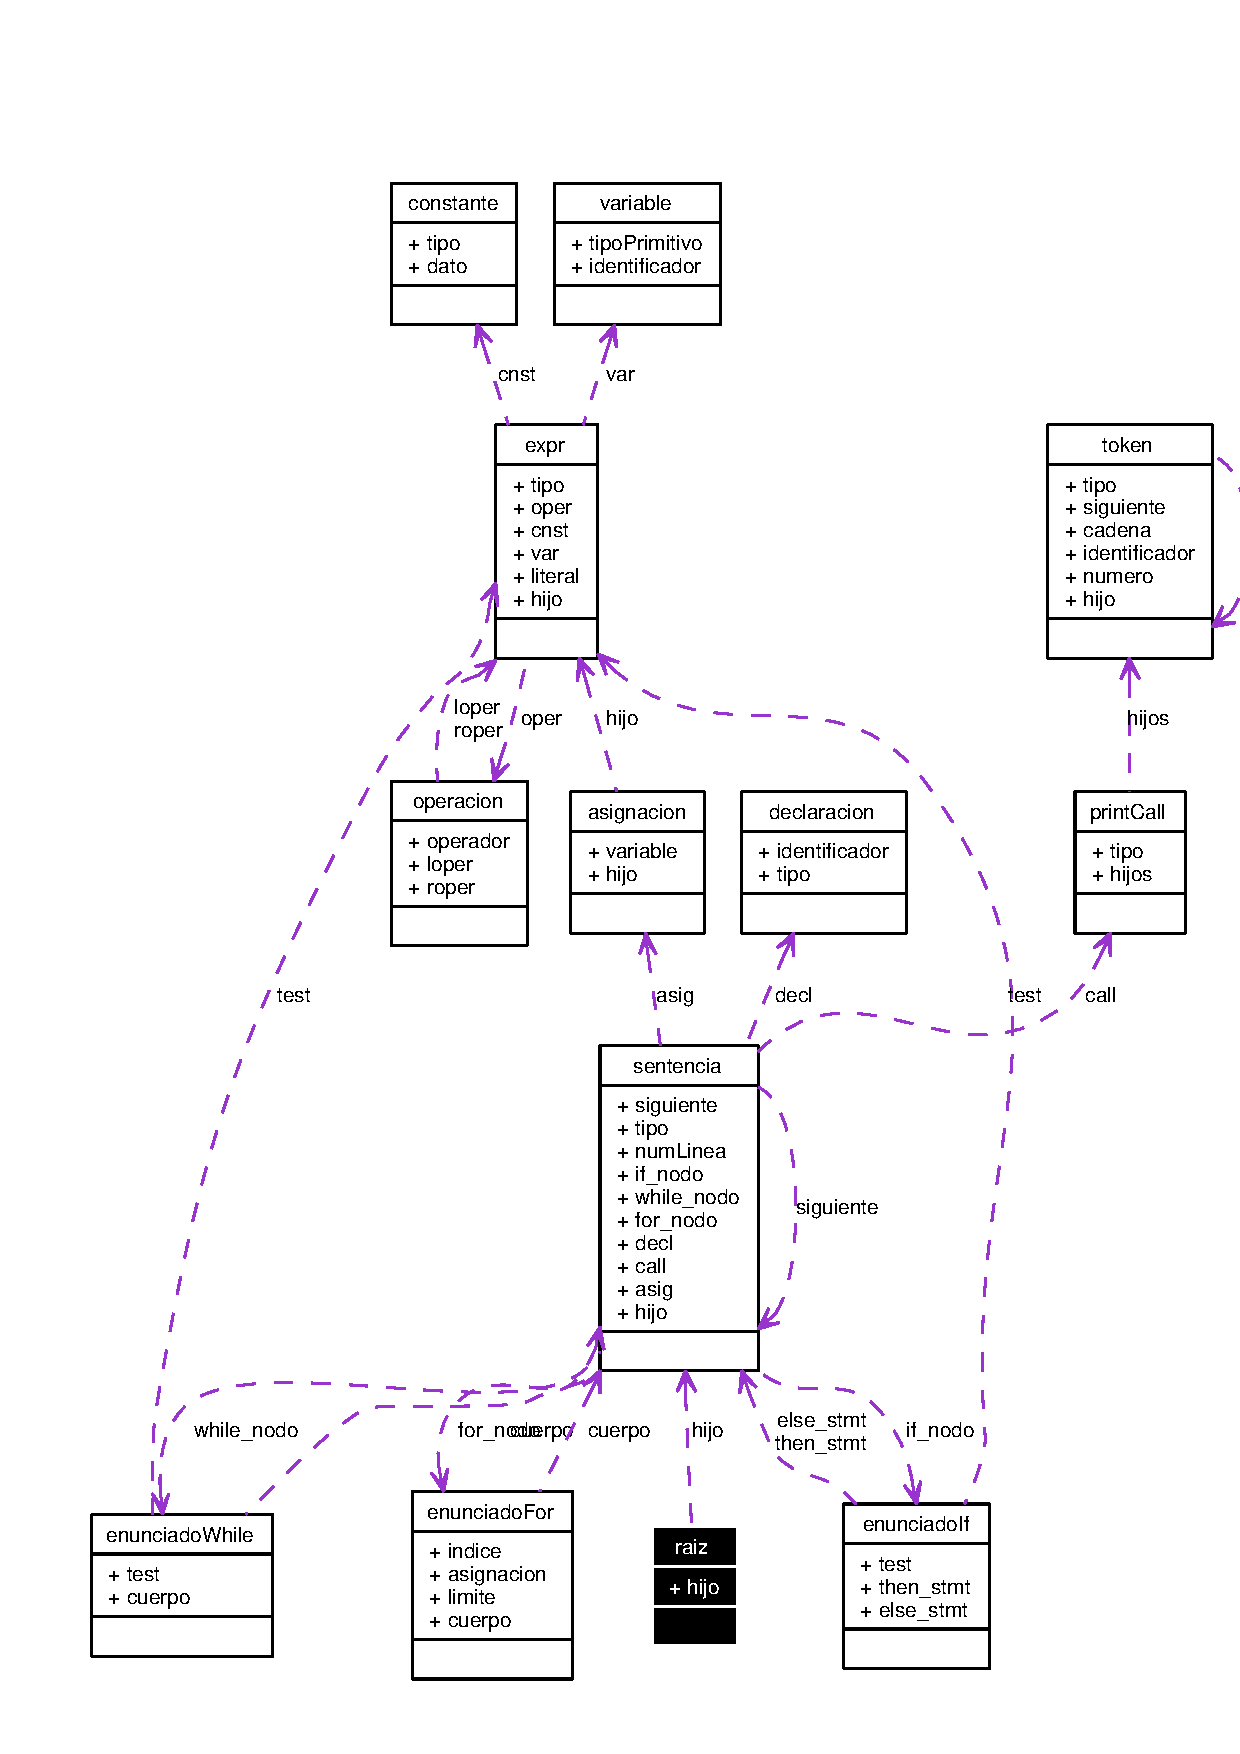
\includegraphics[width=320pt]{structraiz__coll__graph}
\end{center}
\end{figure}
\subsection*{Atributos p\'{u}blicos}
\begin{CompactItemize}
\item 
{\bf sentencia} $\ast$ {\bf hijo}
\begin{CompactList}\small\item\em Primer sentencia del arbol de sintaxis abstracto. \item\end{CompactList}\end{CompactItemize}


\subsection{Descripci\'{o}n detallada}
punto de entrada del AST 



Definici\'{o}n en la l\'{\i}nea 264 del archivo ast.h.

\subsection{Documentaci\'{o}n de los datos miembro}
\index{raiz@{raiz}!hijo@{hijo}}
\index{hijo@{hijo}!raiz@{raiz}}
\subsubsection{\setlength{\rightskip}{0pt plus 5cm}{\bf sentencia}$\ast$ {\bf raiz::hijo}}\label{structraiz_o0}


Primer sentencia del arbol de sintaxis abstracto. 



Definici\'{o}n en la l\'{\i}nea 265 del archivo ast.h.

Referenciado por borrar\-Arbol(), crear\-Raiz(), y recorrer\-Arbol().

La documentaci\'{o}n para esta estructura fu\'{e} generada a partir del siguiente archivo:\begin{CompactItemize}
\item 
/media/docs/progra/c++/compiladores1/proy2/godzilla/src/{\bf ast.h}\end{CompactItemize}
